% !TeX encoding = UTF-8
% !TEX TS-program = xelatex

\documentclass[presentation,aspectratio=1610]{beamer}
%\setbeameroption{show notes}
%\setbeameroption{show notes on second screen=right}

\usetheme{Coventry}
\usepackage{ctex}			 %导入 ctex 宏包,添加中文支持
\usepackage{amsmath,amsfonts,amssymb,bm}
\usepackage{color}
\usepackage{graphicx,hyperref,url}
\usepackage{subfigure}
\usepackage{multirow,makecell}
\usepackage{booktabs}	

\AtBeginSection[]
{
	\begin{frame}<beamer>
	\frametitle{\textbf{目录}}
	\textbf{\tableofcontents[currentsection]}
\end{frame}
}

\title[SIFT \& SURF]{~数~字~图~像~处~理~ \\ SIFT \& SURF简述} 

\author[胡欣毅]{胡欣毅 180776 }
\date[\today]{\today} 

\institute[Coventry] 
{
% 东南大学  \\  \medskip
\small 信息科学与工程学院 \\
\medskip
icedomain\_hu@qq.com

	\begin{flushright}
		2组组长:卞慧	  \\ 
		胡欣毅\qquad \hspace{.02cm}  陈康 \quad  张可涵 \\ 
		包雅孟	 \quad 周京鹏 \quad  郝培钧
	\end{flushright}
}


\begin{document}

\begin{frame}
\titlepage 
\end{frame}

\begin{frame}
\frametitle{目录} 
\tableofcontents

\end{frame}

%----------------------------------------------------------------------------------------
%	PRESENTATION SLIDES
%----------------------------------------------------------------------------------------

\section[SIFT]{尺度不变特征转换(SIFT)}

\begin{frame}
\frametitle{SIFT}
	\begin{block}{\textbf{算法特点}}
		\begin{itemize}
			\item SIFT特征是图像的局部特征,对旋转、尺度缩放、亮度变化保持不变性
			\item 独特性好,信息量丰富,适用于在海量特征数据库中进行快速、准确的匹配
			\item 多量性,即使少数的几个物体也可以产生大量的SIFT特征向量
			\item 高速性,经优化的SIFT匹配算法甚至可以达到实时的要求
			\item 可扩展性,可以很方便的与其他形式的特征向量进行联合
		\end{itemize}
	\end{block} \pause
	
	\begin{block}{\textbf{算法用途}}
		\begin{itemize}
			\item 目标的旋转、缩放、平移(RST)			
			\item 图像仿射/投影变换(视点viewpoint)			
			\item 光照影响(illumination)			
			\item 目标遮挡(occlusion)			
			\item 杂物场景(clutter)			
			\item 噪声
		\end{itemize}
	\end{block}
	
\end{frame}

\begin{frame}
	\frametitle{\textbf{SIFT算法}}
	\begin{columns}
		\column{.5\textwidth}
		尺度空间极值检测
		
	\begin{itemize}
		\item 高斯模糊
		\item 尺度空间极值检测
		\item  高斯金字塔的构建
		\item  空间极值点检测
	\end{itemize}		 \pause
		\column{.5\textwidth}
		关键点定位
		
		\begin{itemize}
			\item 关键点的精确定位
			\item  消除边缘响应
			\item $\dots$
		\end{itemize}	
		
	\end{columns} \vspace{1.0cm} \pause
	
	\begin{columns}
		\column{.5\textwidth}
		方向确定
		\begin{itemize}
			\item 关键点方向分配
			\item $\dots$
		\end{itemize} \pause
		
		\column{.5\textwidth}
		关键点描述
		\begin{itemize}
			\item 关键点特征描述
			\item $\dots$			
		\end{itemize}			
	\end{columns}
\end{frame}

\begin{frame}
	\frametitle{高斯模糊}
	\begin{columns}
		\column{.5\textwidth}
	高斯卷积核是实现尺度变换的唯一变换核,并且是唯一的线性核\\	
	\begin{equation*} 
	G(x, y)=\frac{1}{2 \pi \sigma^{2}} e^{-\frac{(x-m / 2)^{2}+(y-n / 2)^{2}}{2 \sigma^{2}}}
	\end{equation*}	
	
	$\sigma$值越大,图像越模糊(平滑) \vspace{.4cm}
	
	这样进行模糊处理比其它的均衡模糊滤波器更高地保留了边缘效果
	
		\column{.5\textwidth}
		\begin{figure}[htbp!]
			\centering
			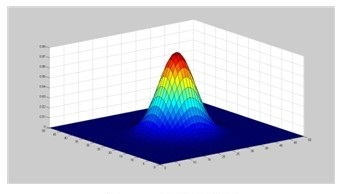
\includegraphics[width=0.9\textwidth]{img/gass.jpg}
		\end{figure}
		
	\end{columns}	
\end{frame}

\begin{frame}
	\frametitle{图像的二维高斯模糊}
	\begin{columns}
		\column{.5\textwidth}
		因模板矩阵的关系而造成边缘图像缺失
		
		\begin{figure}[htbp!]
			\centering
			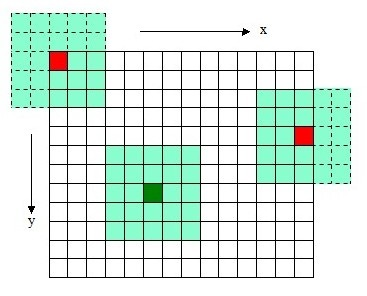
\includegraphics[width=0.8\textwidth]{img/filter1.jpg}
			\caption{5$\times $5的高斯模板卷积}
		\end{figure}	\pause
		\column{.5\textwidth}
		\begin{figure}[htbp!]
			\centering
			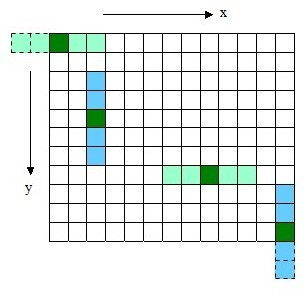
\includegraphics[width=0.7\textwidth]{img/filter2.jpg}
			\caption{1$\times$5分离高斯模糊}
		\end{figure}
		
	\end{columns}	
\end{frame}

\begin{frame}
	\frametitle{高斯金字塔的构建}
	\begin{columns}
		\column{.5\textwidth}
		\footnotesize
		\begin{itemize}
			\item 对图像做不同尺度的高斯模糊
			\item 对图像做降采样(隔点采样)+ 高斯滤波
			\item 金字塔上一组图像的初始图像(底层图像)是由前一组图像的倒数第三张图像隔点采样得到
		\end{itemize}
		
		\begin{figure}[htbp!]
			\centering
			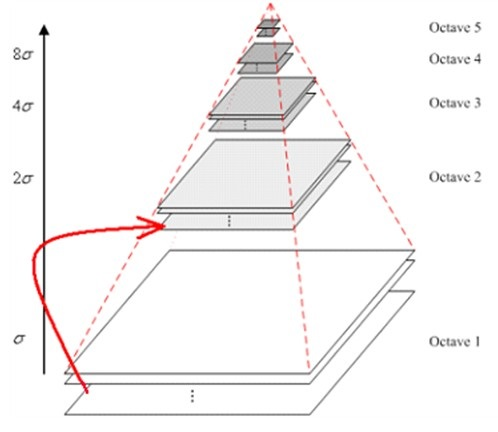
\includegraphics[width=0.8\textwidth]{img/jinzi.jpg}
			\caption{高斯金字塔}
		\end{figure}	\pause
		\column{.5\textwidth}
		\begin{itemize}
			\item {\color{red}{ 尺度规范化的LoG算子具有真正的尺度不变性 }}
			\item \textbf{ Lowe使用高斯差分金字塔近似LoG算子}
		\end{itemize}
		
		\begin{figure}[htbp!]
			\centering
			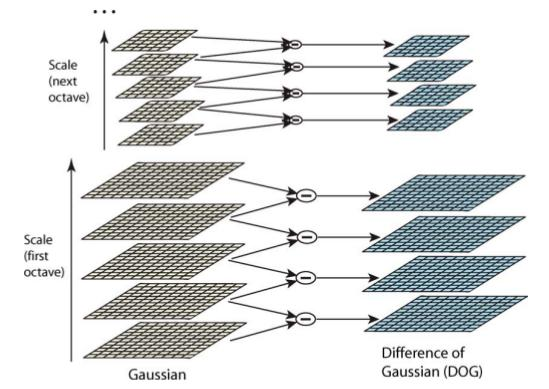
\includegraphics[width=0.9\textwidth]{img/chafen.jpg}
			\caption{高斯差分金字塔}
		\end{figure}
		
	\end{columns}
\end{frame}

\begin{frame}
	\frametitle{极值点检测 \& 关键点定位}
	\begin{columns}
		\column{.5\textwidth}
		同一组内各DoG相邻两层图像之间比较完成
		
	每一个像素点要和它所有的相邻点比较,看其是否比它的图像域和尺度域的相邻点大或者小\\
	\begin{figure}[htbp!]
		\centering
		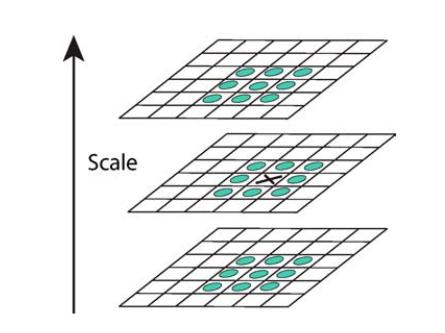
\includegraphics[width=0.9\textwidth]{img/zreo.jpg}
	\end{figure}			
		
		\column{.5\textwidth}
		子像素插值:已知的离散空间点插值得到的连续空间极值点\\
		
	\begin{figure}[htbp!]
		\centering
		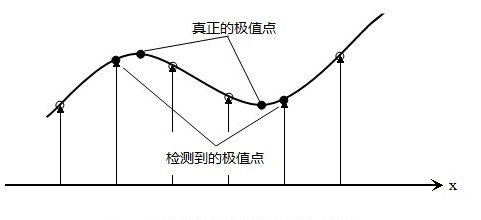
\includegraphics[width=0.9\textwidth]{img/zeros.jpg}
	\end{figure}

\end{columns}

\centering 需要消除“边缘响应”  \quad $\frac{\operatorname{Tr}(\mathbf{H})^{2}}{\operatorname{Det}(\mathbf{H})}<\frac{(r+1)^{2}}{r}$

\end{frame}


\begin{frame}
	\frametitle{关键点方向分配}
	\begin{equation*} 
\begin{aligned} m(x, y) &=\sqrt{(L(x+1, y)-L(x-1, y))^{2}+(L(x, y+1)-L(x, y-1))^{2}} \\ \theta(x, y) &=\tan ^{-1}((L(x, y+1)-L(x, y-1)) /(L(x+1, y)-L(x-1, y))) \end{aligned}
\end{equation*}

	\begin{columns}
		\column{.5\textwidth}
\begin{figure}[htbp!]
	\centering
	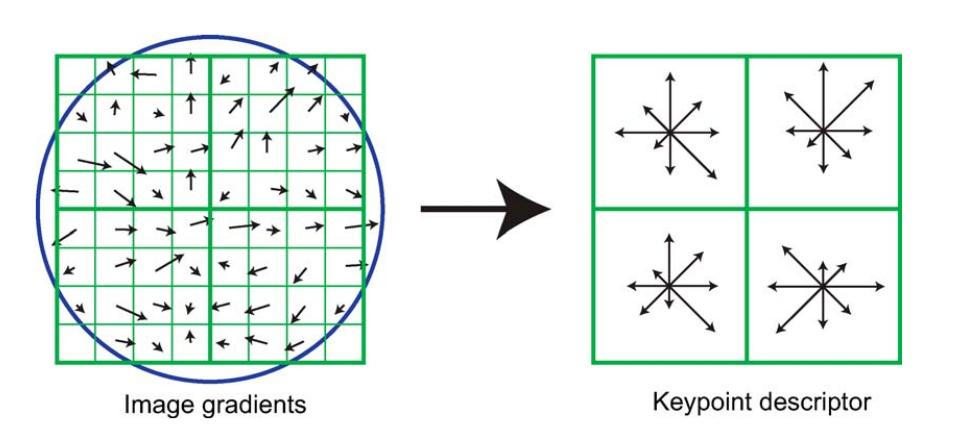
\includegraphics[width=0.9\textwidth]{img/diect.jpg}
	\caption{关键点方向}
\end{figure}
\column{.5\textwidth}
\begin{figure}[htbp!]
	\centering
	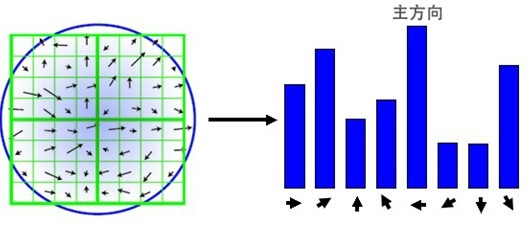
\includegraphics[width=0.9\textwidth]{img/main_diect.jpg}
	\caption{关键点方向直方图}
\end{figure}
	\end{columns} \pause
	保留峰值大于主方向峰值80%的方向作为该关键点的辅方向
\end{frame}


\begin{frame}
	\frametitle{生成关键点特征描述}
	对于每一个关键点,拥有三个信息:位置、尺度以及方向。
	
	为每个关键点建立一个描述符,用一组向量将这个关键点描述出来。\vspace{.9cm}\pause
	
	特征描述符生成的几个步骤:
	\begin{itemize}
		\item 确定计算描述子所需的图像区域 \pause
		\item {\color{red} 校正旋转主方向,确保旋转不变性}\pause
		\item 插值计算每个种子点八个方向的梯度 \pause
		\item {\color{red} 生成描述子,最终形成一个128维的特征向量} \pause
		\item 归一化处理,将特征向量长度进行归一化处理 \pause
		\item 描述子向量门限排除一定干扰 \pause
		\item 按特征点的尺度对特征描述向量进行排序
	\end{itemize}
\end{frame}


\begin{frame}
	\frametitle{生成关键点特征描述}
	\begin{columns}
		\column{.5\textwidth}
		校正旋转主方向
		
	\begin{figure}[htbp!]
		\centering
		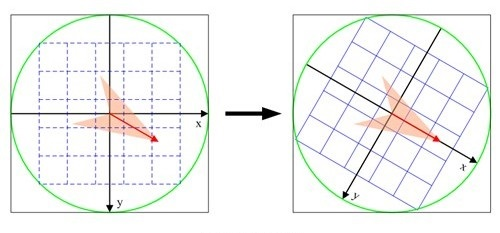
\includegraphics[width=0.9\textwidth]{img/zhuan.jpg}
		\caption{坐标轴选择}
	\end{figure}		
		\column{.5\textwidth}
		生成描述子,最终形成一个128维的特征向量(4$\times$4$\times$8)
		
	\begin{figure}[htbp!]
		\centering
		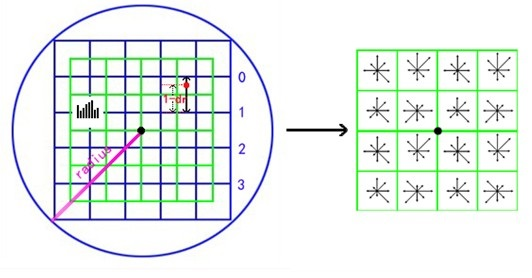
\includegraphics[width=0.9\textwidth]{img/zhifangtu.jpg}
		\caption{描述子梯度}
	\end{figure}	
	\end{columns}
\end{frame}



\section[SURF]{Speeded Up Robust Features(SURF)}
\begin{frame}
	\frametitle{构建Hessian阵}
	金字塔图像的获取
	\begin{itemize}
		\item[sift:] DOG图像
		\item[surf:] Hessian矩阵行列式近似值图像
	\end{itemize}
	 \vspace{.5cm}
	
	每一个像素点都可以求出一个Hessian矩阵	
	
	$$ H(f(x, y))=\left[ \begin{array}{cc}{\frac{\partial^{2} f}{\partial x^{2}}} & {\frac{\partial^{2} f}{\partial x \partial y}} \\ {\frac{\partial^{2} f}{\partial x \partial y}} & {\frac{\partial^{2} f}{\partial x^{2}}}\end{array}\right]$$ \pause
	
	当Hessian矩阵的判别式取得局部极大值(结合下文特征点定位)时,判定当前点是比周围邻域内其他点更亮或更暗的点,由此来定位关键点的位置。
\end{frame}

\begin{frame}
	\frametitle{构建尺度空间}
	不同组间图像的尺寸都是一致的
	
	不同组间使用的盒式滤波器的模板尺寸逐渐增大
	
	同一组间不同层间使用相同尺寸的滤波器,但是滤波器的模糊系数逐渐增大
	
	\begin{figure}[htbp!]
		\centering
		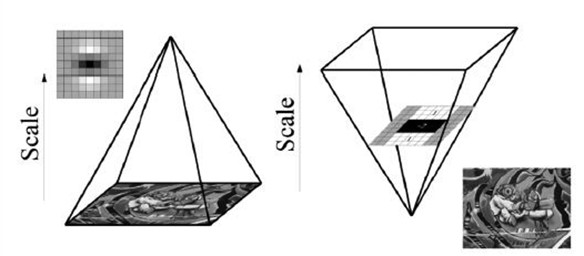
\includegraphics[width=0.7\textwidth]{img/filter3.jpg}
		\caption{盒式滤波器的模板尺寸}
	\end{figure}
\end{frame}


\begin{frame}
	\frametitle{特征点定位}
	\begin{columns}
		\column{.5\textwidth}
	
		特征点的定位过程Surf和Sift保持一致,将经过Hessian矩阵处理的每个像素点与二维图像空间和尺度空间邻域内的26个点进行比较,初步定位出关键点,再经过滤除能量比较弱的关键点以及错误定位的关键点,筛选出最终的稳定的特征点。	
		
		\column{.5\textwidth}
		\begin{figure}[htbp!]
			\centering
			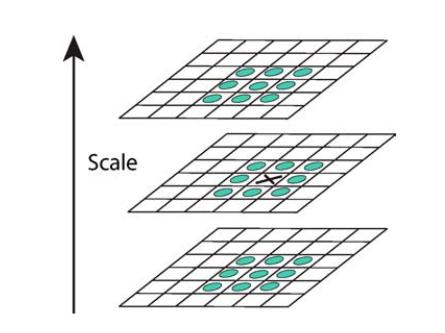
\includegraphics[width=0.9\textwidth]{img/zreo.jpg}
			\caption{特征点定位}
		\end{figure}
	\end{columns}
	
\end{frame}


\begin{frame}
	\frametitle{特征点主方向分配}
		\begin{columns}		
		\column{.5\textwidth}
		\begin{figure}[htbp!]
			\centering
			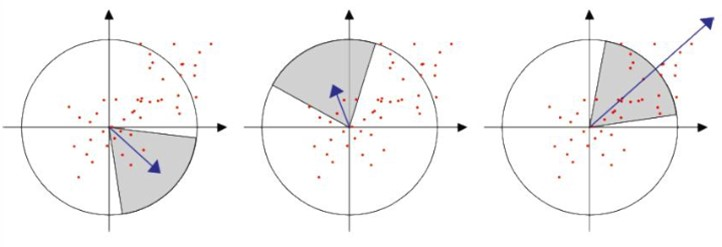
\includegraphics[width=0.9\textwidth]{img/fx.jpg}
			\caption{特征点定位}
		\end{figure}
				
			\column{.5\textwidth}
		采用的是统计特征点圆形邻域内的haar小波特征。\vspace{.5cm}
		
		在特征点的圆形邻域内,统计60度扇形内所有点的水平、垂直haar小波特征总和,然后扇形以一定间隔进行旋转并再次统计该区域内haar小波特征值之后,最后将值最大的那个扇形的方向作为该特征点的主方向。
			
		\end{columns}
\end{frame}

\begin{frame}
	\frametitle{生成特征点描述子}
			\begin{columns}
				\column{.5\textwidth}
				\begin{itemize}
					\item (沿着特征点的主方向)在特征点周围取一个4$\times$4的矩形区域块
					\item 每个子区域统计25个像素的水平方向和垂直方向的haar小波特征(水平和垂直方向相对主方向而言)
					\item 	该haar小波特征为水平方向值之和、垂直方向值之和、水平方向绝对值之和以及垂直方向绝对值之和(4$\times$4$\times$4维描述子)				
				\end{itemize}

				\column{.5\textwidth}
				\begin{figure}[htbp!]
					\centering
					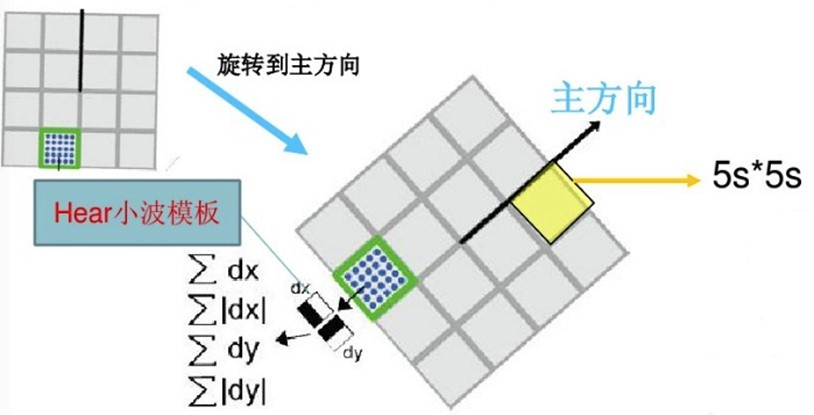
\includegraphics[width=0.9\textwidth]{img/miaoshu.jpg}
					\caption{特征点定位}
				\end{figure}
			\end{columns}
\end{frame}

\begin{frame}
	\frametitle{特征点匹配}
	\begin{enumerate}
		\item[同] Surf也是通过计算两个特征点间的欧式距离来确定匹配度,欧氏距离越短,代表两个特征点的匹配度越好\\
		\item[异] Surf还加入了Hessian矩阵迹的判断
		
		\begin{enumerate}
			\item 两个特征点的矩阵迹正负号相同,代表这两个特征具有相同方向上的对比度变化\\
			\item 两个特征点的矩阵迹正负号不同,说明这两个特征点的对比度变化方向是相反的
		\end{enumerate}
	\end{enumerate}
\end{frame}

\begin{frame}
	\frametitle{对比}
	\begin{itemize}
		\item Sift
	\begin{enumerate}
		\item[优点] 特征稳定,对旋转、尺度变换、亮度保持不变性,对视角变换、噪声也有一定程度的稳定性
		\item[缺点] 实时性不高,并且对于边缘光滑目标的特征点提取能力较弱
	\end{enumerate} \vspace{.5cm}\pause

		\item Surf
			\begin{enumerate}
			\item 改进了特征的提取和描述方式
			\item 用一种更为高效的方式完成特征的提取和描述
		\end{enumerate}
		
	\end{itemize}
\end{frame}


\section[特征匹配]{特征匹配}
\begin{frame}
	\frametitle{SIFT}
	\begin{columns}
		\column{.3\textwidth}
		\begin{figure}[htbp!]
			\centering
			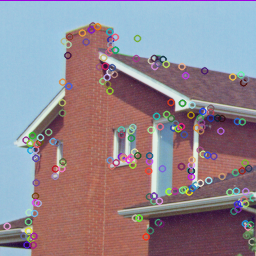
\includegraphics[width=0.9\textwidth]{sift/img_1_feature.png}
		\end{figure}
					
	\begin{figure}[htbp!]
		\centering
		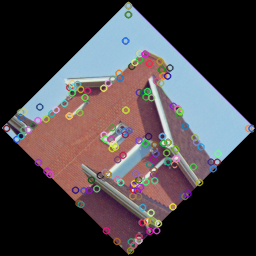
\includegraphics[width=0.9\textwidth]{sift/img_2_feature.png}
	\end{figure}	
		
		\column{.7\textwidth}
		
		\begin{figure}[htbp!]
			\centering
			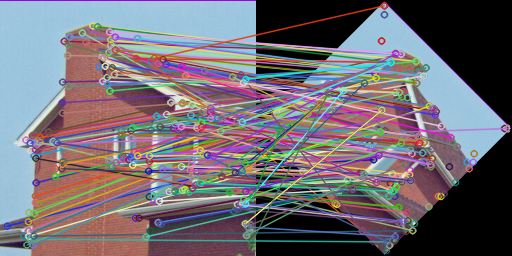
\includegraphics[width=0.7\textwidth]{sift/match1.png}
		\end{figure}
		
		\begin{figure}[htbp!]
			\centering
			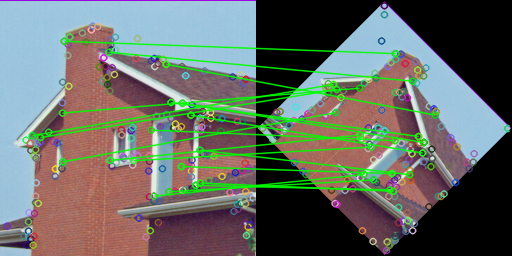
\includegraphics[width=0.7\textwidth]{sift/match2.png}
		\end{figure}
		
	\end{columns}

\end{frame}

\begin{frame}
	\frametitle{SURF}
	\begin{columns}
		\column{.3\textwidth}
		\begin{figure}[htbp!]
			\centering
			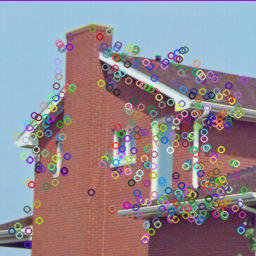
\includegraphics[width=0.9\textwidth]{surf/img_1_feature.png}
		\end{figure}
		
		\begin{figure}[htbp!]
			\centering
			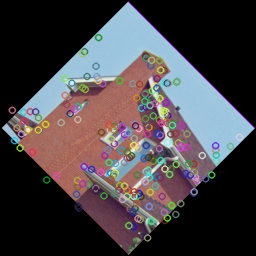
\includegraphics[width=0.9\textwidth]{surf/img_2_feature.png}
		\end{figure}	
		
		\column{.7\textwidth}
		
		\begin{figure}[htbp!]
			\centering
			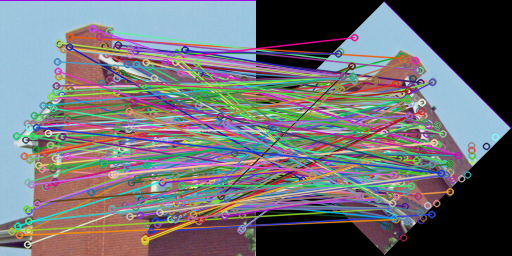
\includegraphics[width=0.7\textwidth]{surf/match1.png}
		\end{figure}
		
		\begin{figure}[htbp!]
			\centering
			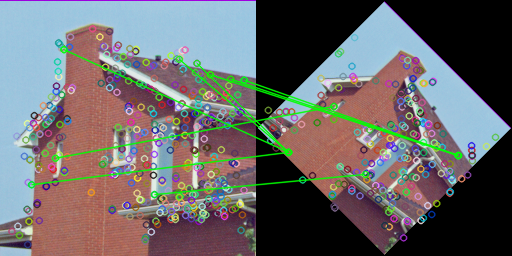
\includegraphics[width=0.7\textwidth]{surf/match2.png}
		\end{figure}
		
	\end{columns}
	
\end{frame}


\section*{}
\begin{frame}
\frametitle{\textbf{}}
\begin{beamercolorbox}[wd=1.0\textwidth, rounded=true, shadow=true]{mybox}
	\Huge \centering \color{covblue} END-ING
\end{beamercolorbox}
\end{frame}


\end{document} 
